\section{Theorie}
\label{sec:Theorie}

\subsection{Brückenspannung und Abgleichbedingung}
Die Spannung $U$, also die Potentialdiffferenz zwischen zwei Punkten, wird bei Brückenschaltungen in Abhängigkeit von ihren 
Widerstandsverhältnissen untersucht.
Bei einer allgemeinen Brückenschaltung (s. Abb \ref{allgemein}), bezeichnet man die Spannung, die zwischen Punkt A und B auftritt, als Brückenspannung. 
$U_S$ wird dabei als Speisespannung bezeichnet.
\begin{figure}
    \centering
    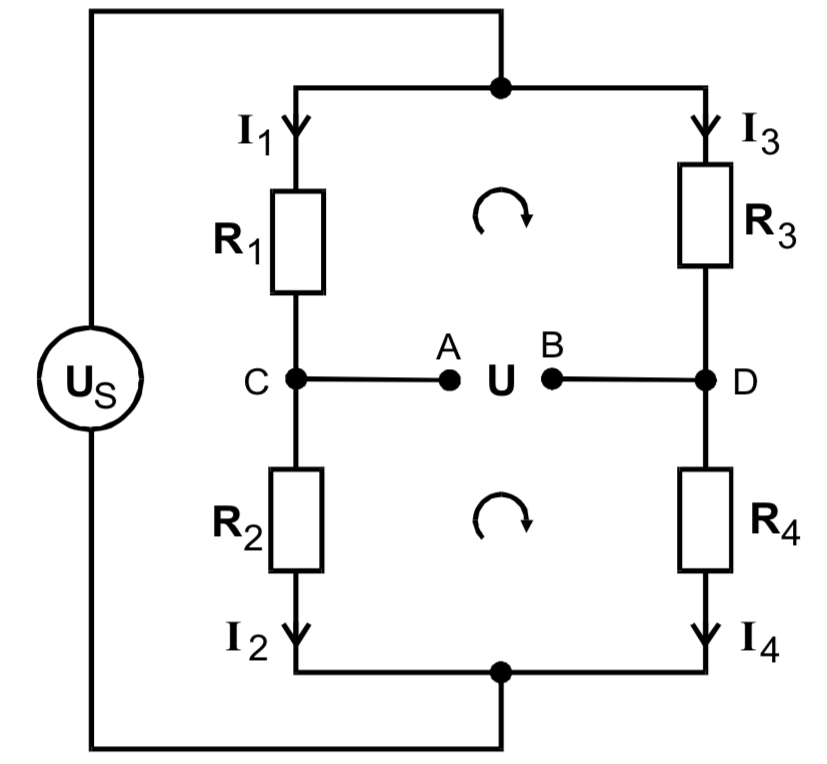
\includegraphics[width=8cm, height=8cm]{build/allgemein.png}
    \caption{Allgemeine Brückenschaltung.}
    \label{allgemein}
\end{figure}
\noindent Wichtig sind dabei die Kirchhoffschen Gesetze. 
Das erste lautet, dass die Summe der zufließenden Ströme gleich der Summe der abfließenden Ströme sein muss. 
Das zweite Gesetzt heißt Maschenregel und besagt, dass innerhalb einer Masche, also einem in sich geschlossenen Stromkreis, die Summe der 
elektromotorischen Kräfte, also zum Beispiel die Spannung der Stromquelle, gleich der Summe aus %den Produkten
der Stromstärke und den Widerständen der Bauteile sein muss. 
\newline
Aus diesen Gesetzmäßigkeiten lässt sich folgern, dass die Brückenspannung $U_B$ und die Speisespannung $U_S$ in Abb. \ref{allgemein} in folgendem Verhältnis 
zueinander stehen:
\begin{equation*}
    U = \frac{R_2R_3 - R_1R_4}{(R_3 + R_4)(R_1 + R_2)}U_S.
\end{equation*}
Eine abgeglichene Brücke ist der Fall, wenn die Brückenspannung verschwindet.
Dies passiert, wenn die Abgleichbedingung
\begin{equation*}
    R_1 R_4 = R_2 R_3
\end{equation*}
gilt.
Da die Abgleichbedingung nur vom Verhältnis der Widerstände abhängt, 
ist mit der Brückenschaltung eine Widerstandsmessung durchführbar. 
Ist ein Widerstand unbekannt, so wird einer der drei anderen Widerstände so lange variiert, bis die Brückenspannung verschwindet. 
Anschließend kann über die Abgleichbedingung der Widerstand bestimmt werden. 
\newline
Bei Kapazitiv- und Induktivwiderständen ist es sinnvoll komplexe Widerstandsoperatoren zu benutzen. %Komma nach "sinnvoll"?
Eine Brückenschaltung mit vier komplexen Widerständen hat die gleiche Abgleichbedingung wie eine reele Brückenschaltung. 
Der einzige Unterschied ist, dass sich daraus zwei Bedingungen ergeben. 
Der Realteil $X$ und der Imaginärteil $Y$ müssen dabei separiert voneinander betrachtet werden. 
Die erste Bedingung ist:
\begin{equation*}
    X_1X_4 - Y_1Y_4 = X_2X_3 - Y_2Y_3.
\end{equation*}
Die zweite Bedingung lautet: 
\begin{equation*}
    X_1Y_4 + X_4Y_1 = X_2Y_3 + X_3Y_2.
\end{equation*}

\subsection{Brückenschaltungen}
\subsubsection{Wheatstonesche Brücke}
Diese Brücke enthält nur ohmsche Widerstände (s. Abb \ref{wheatstone}). Sie kann, wie oben beschrieben, zur Bestimmung eines unbekannten Widerstands $R_X$ benutzt werden:
\begin{equation}
    R_X = R_2 \frac{R_3}{R_4}.
    \label{eqn:a_r}
\end{equation}

\subsubsection{Kapazitätsmessbrücke}
Für die Berechnung muss die Eigenschaft eines realen Kondensators berücksichtigt werden, dass dieser zum Teil Energie in Wärme umwandelt. %real oder reell
Dafür wird ein Ersatzschaltbild betrachtet, bei dem ein fiktiver ohmscher Widerstand mit dem Kondensator in Reihe geschaltet wird. 
Für die Messung der Kapazität eines unbekannten Kondensators $C_X$ gilt somit unter Berücksichtigung der Abgleichbedingungen für den ohmschen 
Widerstand 
\begin{equation}
    R_X = R_2 \frac{R_3}{R_4}
    \label{eqn:b_r}
\end{equation}
und für die Kapazität des Kondensators 
\begin{equation}
    C_X = C_2 \frac{R_4}{R_3}.
    \label{eqn:b_c}
\end{equation}

\subsubsection{Induktivitätsmessbrücke}
Analog zur Kapazitätsmessbrücke verliert auch ein induktives Bauteil Energie, indem diese irreversibel in Wärme umgewandelt wird. 
Diese Verluste und die Phasenverschiebung werden erneut durch einen fiktiven Widerstand kompensiert. 
Die Formeln ergeben sich auf dieselbe Weise zu 
\begin{equation}
    R_X = R_2 \frac{R_3}{R_4}
    \label{eqn:c_r}
\end{equation}
und für die Induktivität zu 
\begin{equation}
    L_X = L_2 \frac{R_3}{R_4}.
    \label{eqn:c_l}
\end{equation}

\subsubsection{Maxwell-Brücke}
Da die Induktivitätsmessbrücke insbesondere bei niedrigen Frequenzen aufgrund der zweiten Spule ähnlich starke Verluste hat, 
wird eine andere Schaltung, die anstelle der Normalinduktivität $L_2$ eine Normalkapazität enthält, benutzt.
Diese Schaltung heißt Maxwell-Brücke (s. Abb \ref{maxwell}).
Der Kondensator sollte eine möglichst verlustarme Kapazität $C_4$ besitzen. 
Aus den Abgleichbedingungen ergeben sich folgende Ausdrücke:
\begin{equation}
     R_X = \frac{R_2R_3}{R_4}
     \label{eqn:d_r}
\end{equation}
und 
\begin{equation}
    L_X = R_2R_3C_4.
    \label{eqn:d_l}
\end{equation}

% \subsection{Frequenzabhängige Brückenschaltungen}
% Bei den vorherigen Schaltungen ist die Frequenz nicht wichtig. 
% Es gibt aber einen Frequenzbereich, in dem der Abgleich unter optimalen Bedingungen durchführbar ist.

\subsubsection{Wien-Robinson-Brücke}
Bei den vorherigen Schaltungen ist die Frequenz nicht wichtig. 
Es gibt aber einen Frequenzbereich, in dem der Abgleich unter optimalen Bedingungen durchführbar ist.
\newline
Die Wien-Robinson-Brücke (s. Abb. \ref{wien-robinson}) ist eine frequenzabhängige Brückenschaltung.
Nach Umformung der Formeln, die sich aus der Abb. \ref{wien-robinson} ergeben, erkennt man, dass
sich ein Verhältnis zwischen den Spannungen $U_B$ und $U_S$ ergibt. 
Es gilt:
\begin{equation}
    \abs{\frac{U_B}{U_S}}^2 = \frac{1}{9} \frac{(\Omega^2 -1)^2}{(1- \Omega)^2 + 9 \Omega^2}.
    \label{eqn:verhaeltnis}
\end{equation}
Dabei ist
\begin{equation}
    \Omega = \frac{\omega}{\omega_0}.
    \label{omega}
\end{equation}
$\omega_0$ ist widerum gegeben durch
\begin{equation}
    \omega_0 = \frac{1}{RC}.
\end{equation}
\newline
Der Klirrfaktor $k$ beschreibt den Oberwellengehalt im Vergleich zur
Grundwelle. Da die Brückenspannung aufgrund von Oberwellen, die durch
den Generator erzeugt werden, bei der Frequenz $f_0$ nicht Null wird,
sondern nur ein Minimum erreicht, ist die Kleinheit des Klirrfaktors
ein Maß für die Qualität eines Spannungsgenerators.
\newline
Es wird angenommen, dass die Summe der Oberwellen aus der zweiten
Oberwelle besteht. Damit ist der Klirrfaktor:
\begin{equation*}
    k = \frac{U_2}{U_1}.
\end{equation*}
$U_2$ ist dabei
\begin{equation*}
    U_2 = \frac{U_B}{n(2)},
\end{equation*}
wobei der Faktor $n(2)$ das Verhältnis \eqref{eqn:verhaeltnis} ist.
Da $\omega = 2 \omega_0$ gilt, ergibt sich für $\Omega$ durch Gleichung \eqref{eqn:omega}
$\Omega = 2$.
Damit wird der Klirrfaktor mittels
\begin{equation}
    k = \frac{U_B}{U_1 \cdot n(2)}. %n(2) berechnen und einsetzen
\end{equation}
berechnet.

% \subsubsection{TT-Brücke}

% Die Funktion ist, genau wie bei der Wien-Robinson-Brücke, die eines elektronischen Filters. 
% Der Vorteil dieser Schaltung ist, dass beide Spannungen gegen Masse angeschlossen werden. 
% Aus den Kirchhoffschen Gesetzen ergibt sich wieder, dass 
% \begin{equation}
%     \omega_0 = \frac{1}{RC}
% \end{equation}
% gilt und dass $U_B$ für $\omega_0$ für diese Frequenz verschwindet, aber sonst von Null verschieden ist. 
% Für den Betrag des Spannungsverhältnisses gilt hierbei 

% \begin{equation}
%     (\frac{U_B}{U_S})^2 = \frac{(\Omega^2 -1)^2}{(1- \Omega^2)^2 + 16 \Omega^2}
% \end{equation}.



